%\PassOptionsToClass{handout}{beamer}
\documentclass[8pt, hyperref={bookmarks=false},aspectratio=169, xcolor=table]{beamer}

% INSERT PREAMBLE FILE (contains all the packages and configurations)
% ------------------------- Packages ---------------------------------

\usepackage[utf8]{inputenc}
\usepackage{multirow,rotating}
\usepackage{color}
\usepackage{hyperref}
\usepackage{tikz-cd}
\usepackage{array}
\usepackage{mathtools,nccmath}%
\usepackage[normalem]{ulem}
\usepackage{pgfplots}
\usepackage{pdfpages}
\usepackage[absolute,overlay]{textpos}
\usepackage{fontawesome}
\usepackage{outlines}
\usepackage[11pt]{moresize}
\usepackage{datetime}
\usepackage{tabularx}
\usepackage[numbers]{natbib}
\usepackage{pgfpages}
\usepackage{appendixnumberbeamer}
\usepackage{appendix}
\usepackage{adjustbox}
\usepackage{multimedia}

% ------------------------ Settings -------------------------------
\useunder{\uline}{\ul}{}

\usetikzlibrary{matrix, decorations.pathreplacing}
\usetikzlibrary{shapes,backgrounds}
\usetikzlibrary{arrows}
\usetikzlibrary{shapes.geometric}
\usetikzlibrary{calc}
\usetikzlibrary{positioning}
\usetikzlibrary{intersections}

\newcommand*{\graybullet}{\textcolor{gray}{\textbullet}}
\newcommand*{\bluebullet}{\textcolor{blue}{\textbullet}}
\newcommand*{\redbullet}{\textcolor{red}{\textbullet}}


% ---------------  Define theme and color scheme  -----------------
\usetheme[minimal]{IFR}  % 2 options: minimal, sidebarleft

\setbeamercovered{transparent} 

\makeatletter
\AtBeginDocument{%
  \let\@biblabel\NAT@biblabelnum
  \let\@bibsetup\NAT@bibsetnum}
\makeatother

\hypersetup{
  colorlinks=true,
  citecolor=black
}

\setbeamerfont{block title}{size=\normalsize}
\setbeamerfont{block body}{size=\small}

% ------------------------- Theorem environments -------------------

\newtheorem{remark}{Remark}
\newtheorem{algorithm}{Algorithm}
\newtheorem{conferences}{Conferences}
\newtheorem{assumptions}{Assumptions}

\AtBeginEnvironment{conferences}{%
  \setbeamercolor{block title}{use=example text,bg=orange!90!yellow}
  \setbeamercolor{block body}{parent=normal text,use=block title example}
}

\AtBeginEnvironment{remark}{%
  \setbeamercolor{block title}{use=example text,bg=Green!70!black}
  \setbeamercolor{block body}{parent=normal text,use=block title example}
}

\AtBeginEnvironment{definition}{%
  \setbeamercolor{block title}{use=example text,bg=orange!90!yellow}
  \setbeamercolor{block body}{parent=normal text,use=block title example}
}

\mode<handout>{%
  \pgfpagesuselayout{2 on 1}[a4paper] 
  \setbeameroption{show notes}
}









% INSERT CONFIG FILE (contains all the basic information about the presentation) 
% -----------------  Information about the presentation  --------------------

% INSERT TITLE HERE
\def\title{\LARGE Region of attraction with integral quadratic constraints}

% INSERT SUBTITLE HERE
\def\subtitle{\small \textit{\today}}

% INSERT AUTHOR HERE
\def\shortauthor{First Last}

% CREATE COMMAND with biography info
\newcommand{\insertbioINFO}{%
    \textbf{\shortauthor}\\[0.2cm]
    E-Mail: \ldots@ifr.uni-stuttgart.de
}

% you can use this line to insert a photo of the speaker (This image appear in the Bio)
%\pgfdeclareimage[width=2.5cm]{speaker}{figures/photo_iFR.png} 
\pgfdeclareimage[width=1.5cm]{speaker}{figures/logo_ifr.png}

% this logo appears in the bio page
\pgfdeclareimage[height=1cm]{unilogow}{figures/unilogo_w.pdf} 

% this logo appears in the title page on the top left corner
\pgfdeclareimage[height=3cm]{unilogoger}{figures/unistuttgart_logo_englisch.pdf}

\AtBeginSection[]
{
  \begin{frame}
    \frametitle{Today's Agenda}
    % Shows the current and previously visited sections normally, hiding future ones
    \tableofcontents[sections={1-\arabic{section}}]
  \end{frame}
}

% ---------------------------- BEGIN DOCUMENT ------------------------------

\begin{document}

\setbeamertemplate{mini frame}{%
  \begin{pgfpicture}{0pt}{0pt}{0.1cm}{0.1cm}
    \pgfsetfillcolor{red} % Use the custom color here
    \pgfpathcircle{\pgfpoint{0.05cm}{0.05cm}}{0.05cm}
    \pgfusepath{fill,stroke}
  \end{pgfpicture}%
}

% INSERT TITLE PAGE

% Set the color of hyperlinks (e.g., TOC links, URLs) to white so they are not visible
\hypersetup{
  colorlinks=white,
  linkcolor=white,     % Color of internal links (e.g., section references)
  urlcolor=white       % Color of URLs
}

% Create a full-screen frame without any standard header/footer
\begin{frame}[plain]
  % Overlay allows drawing over the whole slide
  \begin{tikzpicture}[overlay, remember picture]

  % Define two points A and B to span the area for the background rectangle
  \node[] (A) at (-2.5,2){};    % Top-left corner of the background
  \node[] (B) at (15, -4){};    % Bottom-right corner of the background

  % Draw a large blue rectangle for the background
  \fill[color=renatoSblue!90] (A) rectangle (B);

  % Insert the hexacopter image at a fixed position relative to point A
  \node[anchor=north west, xshift= 0cm, yshift=0.4cm] at ($(A)+(8,0)$) {
    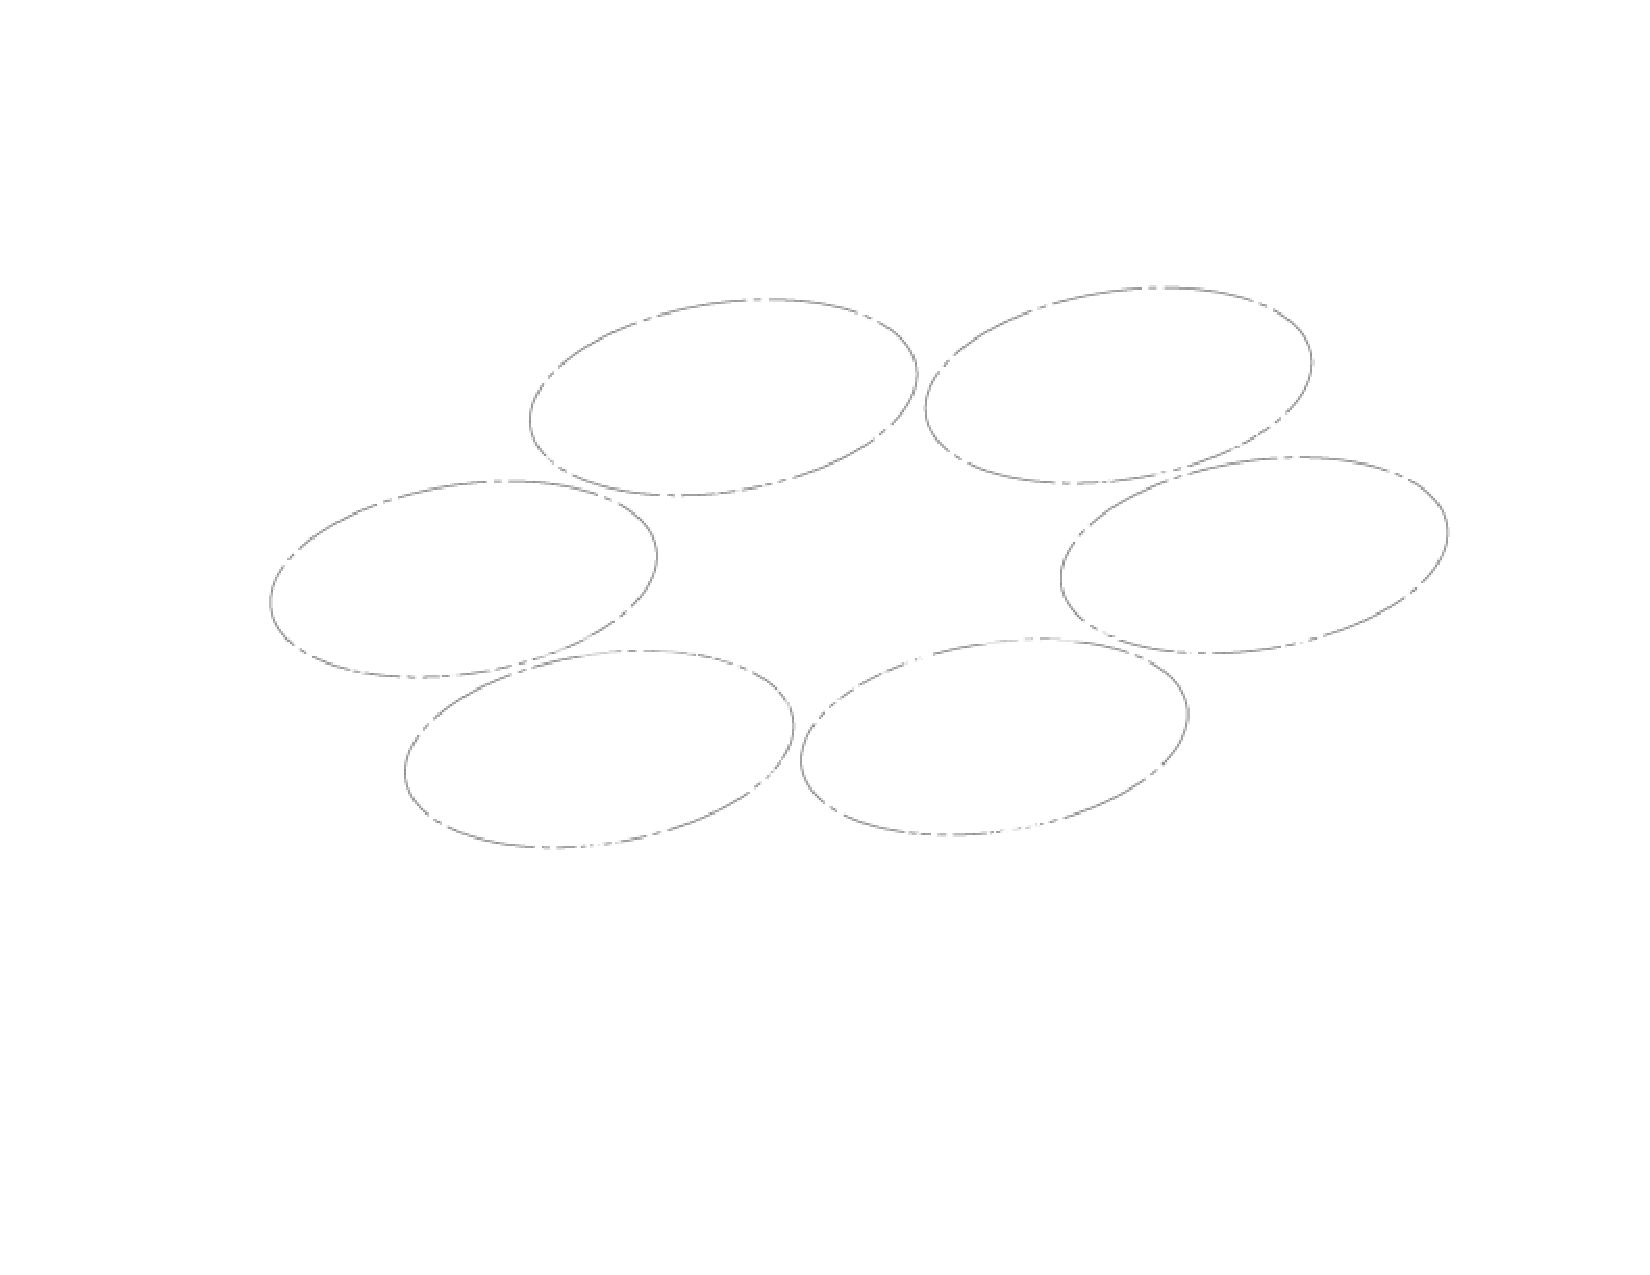
\includegraphics[width=0.7\textwidth]{figures/hexacopter_white.pdf}
  };

  % Insert the University of Stuttgart logo at the top-left of the slide
  \node[anchor=north west] (UNI) at ([xshift=0.5cm, yshift=-2cm]current page.north west) {\pgfuseimage{unilogow}};
  
  % Add the name of the institute next to the logo
  \node[text=white, font=\normalsize, anchor=west] at ($(UNI.west) + (1.25,-0.35)$) {Institut für Flugmechanik und Flugregelung};  
    
  % Insert the title at the bottom-left of the slide
  \node[text=white, anchor=west] at ([yshift=4cm, xshift=0.5cm]current page.south west) {
    \begin{minipage}{0.5\textwidth}
      \raggedright \title   % Title variable
    \end{minipage}  
  };
  
  % Add a subtitle line
  \node[text=white, font=\small, anchor=west] at ([yshift=3.2cm, xshift=0.5cm]current page.south west) {System Theoretical Methods for Flight Control};  

  % Add the actual subtitle defined by \subtitle
  \node[text=white, font=\huge, anchor=west] at ([yshift=2.8cm, xshift=0.5cm]current page.south west) {\subtitle};  
  
  % Add the short author name defined by \shortauthor
  \node[text=white, font=\large, anchor=west] at ([yshift=2.2cm, xshift=0.5cm]current page.south west) {\shortauthor};

  \end{tikzpicture}
\end{frame}

% Set Beamer color for frame titles in the rest of the document
\setbeamercolor{frametitle}{fg=Blue,bg=LightGrey}

% ---------------------------- Content -------------------------------------

% color of links
\hypersetup{
  colorlinks=on,
  linkcolor=black,     % Color of internal links
  urlcolor=black       % Color of URLs
}

\begin{frame}\frametitle{Outline}
  \tableofcontents
\end{frame}

%---------------------------------------------------------
\section{Introduction}
%---------------------------------------------------------
\begin{frame}\frametitle{Motivation for Data-Driven Control}
  \begin{itemize}
    \item \textbf{Bypassing System Identification:} Directly design controllers from experimental data without needing a highly accurate parametric model.
    \item \textbf{Handling Complexity:} Highly effective for systems with dynamics that are notoriously difficult to model from first principles (e.g., complex aerodynamics, friction).
    \item \textbf{Reducing Modeling Errors:} Mitigates performance and safety degradation caused by unmodeled dynamics or model-reality mismatches.
    \item \textbf{Time and Cost Efficiency:} Saves the significant engineering time and effort usually required to build and validate mathematical models.
  \end{itemize}
\end{frame}

%---------------------------------------------------------
\begin{frame}\frametitle{Different Approaches for Data-Driven Control}
  \centering
  \vspace{0.5cm}
  \begin{adjustbox}{max width=\textwidth}
  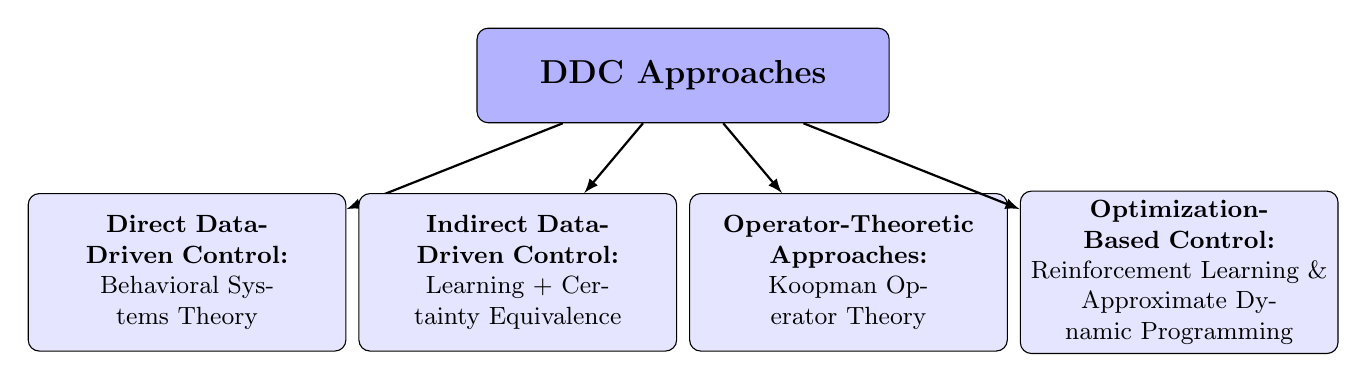
\begin{tikzpicture}[
    level 1/.style={sibling distance=4.2cm, level distance=2.5cm},
    edge from parent/.style={draw, -latex, thick},
    box/.style={draw, rounded corners, align=center, minimum height=2cm, text width=3.8cm, fill=blue!10, font=\small},
    root/.style={draw, rounded corners, align=center, minimum height=1.2cm, text width=5cm, fill=blue!30, font=\bfseries\large}
  ]
    \node[root] {DDC Approaches}
      child { node[box] {\textbf{Direct Data-Driven Control:}\\ Behavioral Systems Theory} }
      child { node[box] {\textbf{Indirect Data-Driven Control:}\\ Learning + Certainty Equivalence} }
      child { node[box] {\textbf{Operator-Theoretic Approaches:}\\ Koopman Operator Theory} }
      child { node[box] {\textbf{Optimization-Based Control:}\\ Reinforcement Learning \& \\Approximate Dynamic Programming} };
  \end{tikzpicture}
  \end{adjustbox}
\end{frame}

%---------------------------------------------------------
\begin{frame}\frametitle{Different Approaches for Data-Driven Control}
  \centering
  \vspace{0.2cm}
  \begin{adjustbox}{max width=0.9\textwidth}
  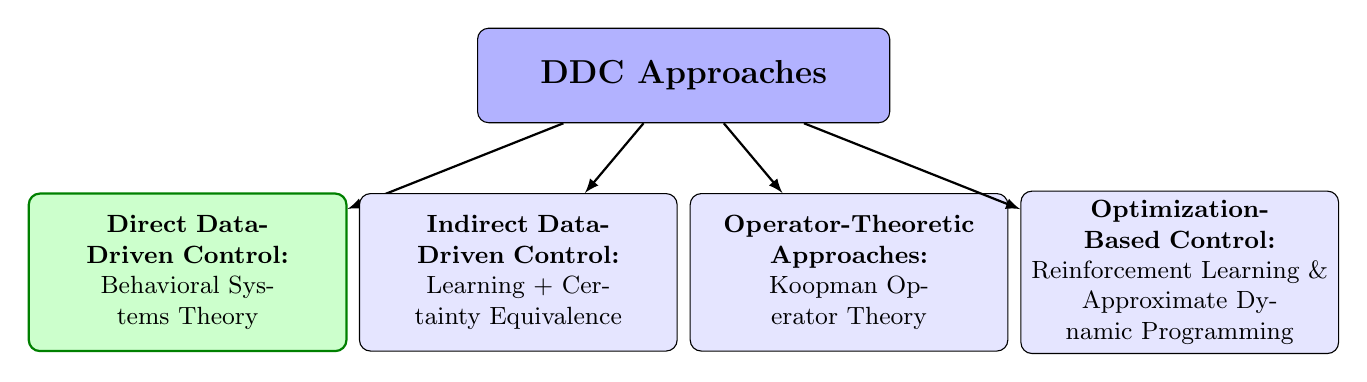
\begin{tikzpicture}[
    level 1/.style={sibling distance=4.2cm, level distance=2.5cm},
    edge from parent/.style={draw, -latex, thick},
    box/.style={draw, rounded corners, align=center, minimum height=2cm, text width=3.8cm, fill=blue!10, font=\small},
    root/.style={draw, rounded corners, align=center, minimum height=1.2cm, text width=5cm, fill=blue!30, font=\bfseries\large}
  ]
    \node[root] {DDC Approaches}
      child { node[box, fill=green!20, draw=green!50!black, thick] {\textbf{Direct Data-Driven Control:}\\ Behavioral Systems Theory} }
      child { node[box] {\textbf{Indirect Data-Driven Control:}\\ Learning + Certainty Equivalence} }
      child { node[box] {\textbf{Operator-Theoretic Approaches:}\\ Koopman Operator Theory} }
      child { node[box] {\textbf{Optimization-Based Control:}\\ Reinforcement Learning \& \\Approximate Dynamic Programming} };
  \end{tikzpicture}
  \end{adjustbox}
  
  \vspace{0.5cm}
  \begin{itemize}
    \item \textbf{Specific Methods Used in This Paper for Robustness:}
    \begin{itemize}
      \item \textbf{Density Functions:} Serve as safety certificates to prove the system avoids unsafe regions.
      \item \textbf{Bounded Process Noise:} Explicitly accounts for unknown but bounded experimental noise/disturbances.
      \item \textbf{Convex Optimization (SDP):} Reformulates non-convex safety constraints into tractable Semidefinite Programs.
      \item \textbf{Sum-of-Squares (SOS):} Relaxes polynomial inequalities to solve the SDP computationally.
    \end{itemize}
  \end{itemize}
\end{frame}

%---------------------------------------------------------
\begin{frame}\frametitle{Goal of the Paper}
  \textbf{Nonlinear System Setup:}
  \begin{equation*}
    \dot{\mathbf{x}}(t) = f(\mathbf{x}(t)) + g(\mathbf{x}(t)) \mathbf{u}(t) + \mathbf{w}(t)
  \end{equation*}
  \begin{itemize}
    \item State $\mathbf{x} \in \mathcal{X} \subset \mathbb{R}^n$, Input $\mathbf{u} \in \mathcal{U} \subset \mathbb{R}^m$
    \item Unknown true dynamics $f(\mathbf{x})$ and $g(\mathbf{x})$ (only noisy data is available)
    \item Unknown but bounded process noise/disturbance $\mathbf{w}(t) \in \mathcal{W}$
  \end{itemize}
  
  \vspace{0.3cm}
  \begin{block}{Intended Results (Robust Safety Objective)}
    Synthesize a state feedback control law $\mathbf{u} = k(\mathbf{x})$ directly from data such that:
    \begin{itemize}
      \item The closed-loop system is \textbf{robustly safe}.
      \item Trajectories starting in an initial set $\mathcal{X}_0$ \textbf{never} enter an unsafe region $\mathcal{X}_u$, despite any allowable disturbance $\mathbf{w} \in \mathcal{W}$.
    \end{itemize}
  \end{block}
\end{frame}

%---------------------------------------------------------
\section{Traditional Approach \& its Challenges}
%---------------------------------------------------------
\begin{frame}\frametitle{Traditional Approach}
  Traditionally, robustness and safety verification are achieved through barrier certificates \cite{Prajna2004}. 
  
  \vspace{0.3cm}
  \textbf{Barrier Functions for Safety:}
  \begin{itemize}
    \item A barrier function $B(\mathbf{x})$ separates safe states from unsafe states $\mathcal{X}_u$.
    \item \textbf{Condition:} $B(\mathbf{x}) > 0$ for $\mathbf{x} \in \mathcal{X}_u$ and $B(\mathbf{x}) \le 0$ for safe initial states $\mathcal{X}_0$.
    \item To ensure trajectories never enter $\mathcal{X}_u$, the derivative along the system dynamics must satisfy:
  \end{itemize}
  
  \begin{equation*}
    \dot{B}(\mathbf{x}) = \frac{\partial B(\mathbf{x})}{\partial \mathbf{x}} \left( f(\mathbf{x}) + g(\mathbf{x})\mathbf{u} + \mathbf{w} \right) \le 0 \quad \text{on the boundary of the safe set}
  \end{equation*}

  \vspace{0.1cm}
  \begin{block}{The Challenge}
    Jointly searching for a barrier certificate $B(\mathbf{x})$ and a control policy $\mathbf{u} = k(\mathbf{x})$ from data inherently results in a \textbf{non-convex optimization problem} (due to the multiplication of the two unknowns).
  \end{block}
\end{frame}

%---------------------------------------------------------
\section{Proposed Solution \& its Advantage}
%---------------------------------------------------------
\begin{frame}\frametitle{Proposed Solution}
  To overcome the non-convexity of barrier functions, the proposed framework uses \textbf{Density Functions} $\rho(\mathbf{x})$ as an alternative safety certificate.
  
  \vspace{0.3cm}
  \textbf{Key Idea (Dual to Lyapunov/Barrier):}
  \begin{itemize}
    \item Instead of preventing trajectories from crossing a strict boundary, density functions prove that the "flow" of trajectories diverges away from the unsafe set $\mathcal{X}_u$.
    \item Safety is guaranteed by verifying a linear partial differential inequality on $\rho(\mathbf{x})$.
  \end{itemize}
  
  \vspace{0.3cm}
  \begin{block}{Convexifying the Synthesis Problem}
    By introducing a change of variables $\mathbf{v}(\mathbf{x}) = \rho(\mathbf{x}) \mathbf{u}(\mathbf{x})$, the bilinear coupling of the unknown certificate and the unknown controller becomes \textbf{linear}.
    \begin{equation*}
      \rho(\mathbf{x}) \mathbf{u}(\mathbf{x}) \text{ (non-convex)} \quad \longrightarrow \quad \mathbf{v}(\mathbf{x}) \text{ (convex)}
    \end{equation*}
  \end{block}
\end{frame}

%---------------------------------------------------------
\begin{frame}\frametitle{Deriving the SDP Formulation}
  Since the true continuous-time dynamics are unknown, we rely directly on the collected noisy experimental data and the known noise bounds.

  \vspace{0.3cm}
  \textbf{From Data to Semidefinite Programming (SDP):}
  \begin{itemize}
    \item \textbf{Polynomial Assumptions:} The system dynamics, density function $\rho(\mathbf{x})$, and controller $\mathbf{v}(\mathbf{x})$ are parameterized as polynomials.
    \item \textbf{Robust Constraints:} The safety condition must hold for all possible disturbances $\mathbf{w} \in \mathcal{W}$ that are consistent with the data.
    \item \textbf{Sum-of-Squares (SOS) Relaxation:} The strict polynomial non-negativity conditions are relaxed into SOS conditions, which are computationally tractable.
  \end{itemize}

  \vspace{0.2cm}
  \begin{block}{Resulting Optimization}
    The robust safety constraints are reformulated into Linear Matrix Inequalities (LMIs) using the data. The entire synthesis problem is solved as a \textbf{Semidefinite Program (SDP)}.
  \end{block}
\end{frame}

%---------------------------------------------------------
\begin{frame}\frametitle{Advantages Over Traditional Approaches}
  The proposed density-function framework provides several distinct advantages:

  \vspace{0.3cm}
  \begin{itemize}
    \item \textbf{Convex Optimization:} Transforms a notoriously difficult non-convex problem (jointly finding a certificate + controller) into a convex SDP, guaranteeing a global optimum.
    \item \textbf{Tractable Robustness:} Incorporating bounded process noise mathematically translates into robust LMI conditions, cleanly handled by SOS without making the problem unsolvable.
    \item \textbf{Directly Data-Driven:} Sidesteps the need to identify the exact nonlinear model first, which is often highly sensitive to modeling errors.
    \item \textbf{Rational Controller:} The resulting state feedback law $\mathbf{u}(\mathbf{x}) = \frac{\mathbf{v}(\mathbf{x})}{\rho(\mathbf{x})}$ is a rational function, allowing for highly flexible and expressive control policies.
  \end{itemize}
\end{frame}

%---------------------------------------------------------
\section{Implementation}
%---------------------------------------------------------
\begin{frame}\frametitle{Implementation}
  Casos tool for controller and observer synthesis
\end{frame}

%---------------------------------------------------------
\section{Validation}
%---------------------------------------------------------
\begin{frame}\frametitle{Validation}
  Experimental verification and performance analysis
\end{frame}

%---------------------------------------------------------
\section{TikZ Examples}
%---------------------------------------------------------

\begin{frame}\frametitle{Awesome TikZ}
  % telling how nice tikz is
  \centering
  \begin{adjustbox}{width=0.35\linewidth}
  
\begin{tikzpicture}
    \node[draw,circle,minimum size=2cm,inner sep=0pt, align=center, font=\bfseries, fill={rgb:red,0;green, 7.5;blue,10}, text=white] at (6.5,-0.5) {TikZ \\ is \\ awesome};
  \end{tikzpicture}
  \end{adjustbox}\\
  \vspace{0.1cm}
  \large In the next slides, we will see some examples.
\end{frame}

%--------------------------------------------------------

\begin{frame}\frametitle{TikZ Example - 1}

  \centering
  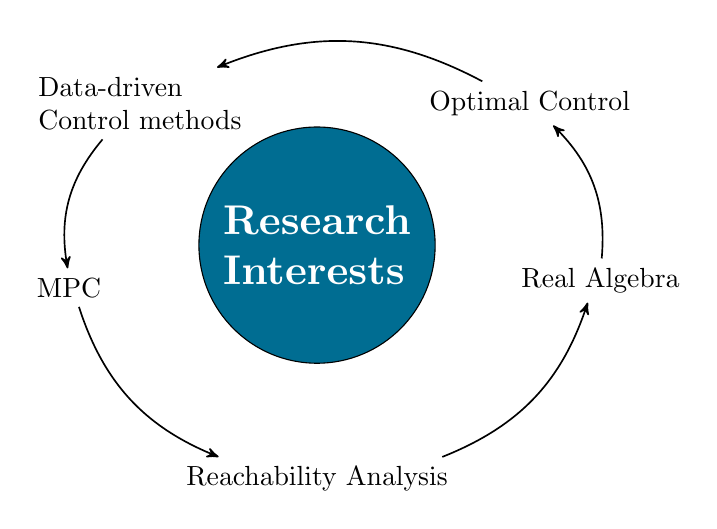
\begin{tikzpicture}[scale=0.9]
    \node[draw,circle,minimum size=2cm,inner sep=0pt, align=left, font=\bfseries, fill={rgb:red,0;green, 7.5;blue,10}, text=white, scale=1.5] at (6.5,-0.5) {Research \\Interests};

    \node[text=black, font=\normalsize, align=left] (ra) at (10.5,-1) {Real Algebra};

    \node[text=black, font=\normalsize, align=left] (reach) at (6.5,-3.8) {Reachability Analysis};

    \node[text=black, font=\normalsize, align=left] (mpc) at (3,-1.1) {MPC};

    \node[text=black, font=\normalsize, align=left] (oc) at (9.5,1.5) {Optimal Control};

    \node[text=black, font=\normalsize, align=left] (ddc) at (4,1.5) {Data-driven \\Control methods};

    %\pause

    \draw[->,>=stealth',semithick] (ra) to[bend right=25] (oc);
    \draw[->,>=stealth',semithick] (oc) to[bend right=25] (ddc);
    \draw[->,>=stealth',semithick] (ddc) to[bend right=25] (mpc);
    \draw[->,>=stealth',semithick] (mpc) to[bend right=25] (reach);
    \draw[->,>=stealth',semithick] (reach) to[bend right=25] (ra);

  \end{tikzpicture}
\end{frame}

%--------------------------------------------------------

\begin{frame}\frametitle{TikZ Example - 2}
  \centering
  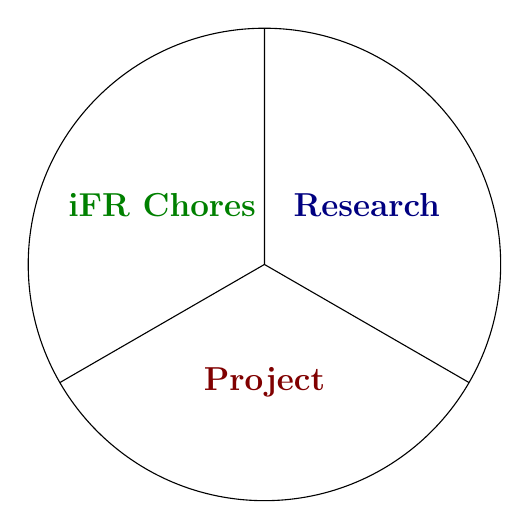
\begin{tikzpicture}
    \draw (0,0) circle (3);
            \draw (0,3) -- (0,0) -- (3*0.866,-3*0.5) (0,0) -- (-3*0.866,-3*0.5);
            \node[text=red!50!black, font=\bfseries\large, align=left] at (0,-1.5) {\textbf{Project}};
            \node[text=blue!50!black, font=\bfseries\large, align=left] at (1.5*0.866,1.5*0.5) {\textbf{Research}};
            \node[text=green!50!black, font=\bfseries\large, align=left] at (-1.5*0.866,1.5*0.5) {\textbf{iFR Chores}};
    \end{tikzpicture}
\end{frame}

%--------------------------------------------------------

\begin{frame}\frametitle{TikZ Example - 3}
  \begin{figure}[H]
      \centering
      \begin{adjustbox}{width=0.5\linewidth}
      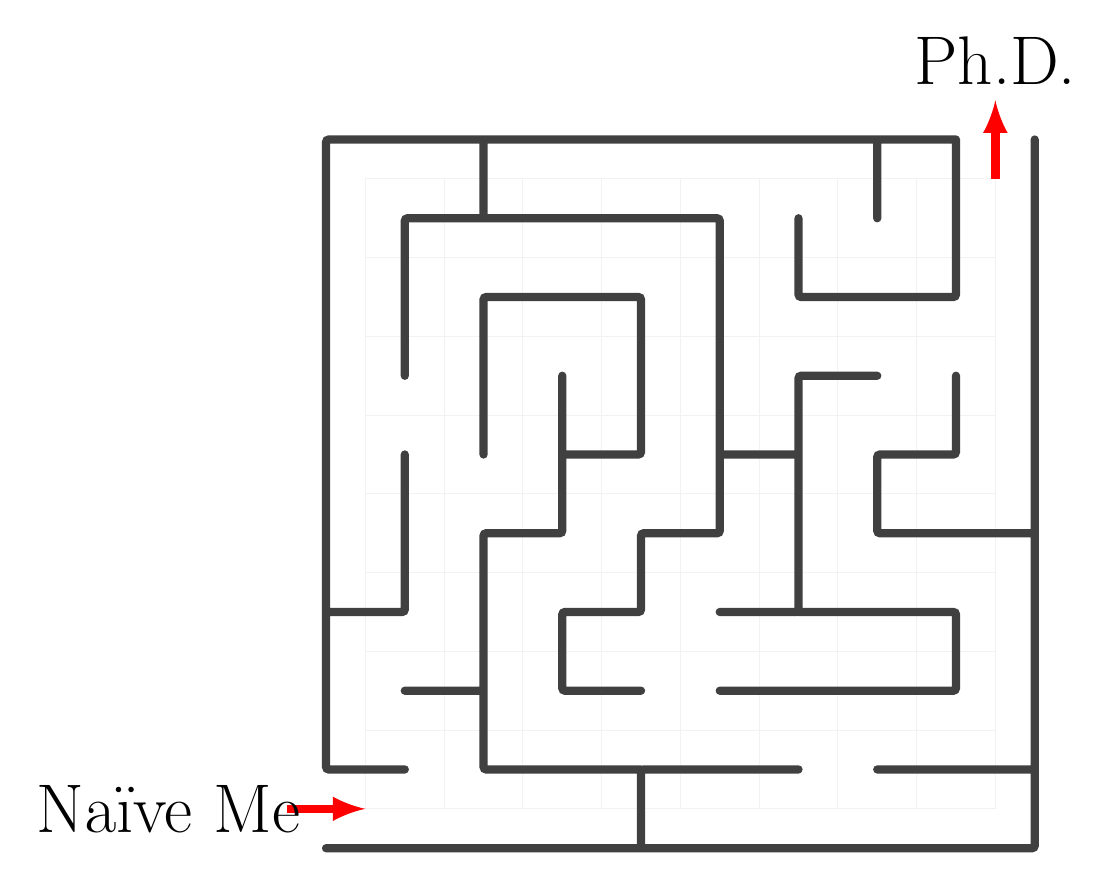
\begin{tikzpicture}
        % Grid
        \draw[lightgray!20] (0,0) grid (8,8);

        % Puzzle
        \draw[line width=3pt, cap=round, rounded corners=1pt, draw=black!75] (-0.5,-0.5) -| (8.5,8.5)
        (7.5,8.5)-|(-0.5,0.5) -- (0.5,0.5) (-0.5,2.5)-|(0.5,4.5)
        (0.5,5.5)|-(4.5,7.5)|-(3.5,3.5)|-(2.5,2.5)|-(3.5,1.5)
        (8.5,0.5)--(6.5,0.5)
        (5.5,0.5)-|(3.5,-0.5)
        (3.5,0.5)-|(1.5,3.5)-|(2.5,5.5)
        (2.5,4.5)-|(3.5,6.5)-|(1.5,4.5)
        (7.5,8.5)|-(5.5,6.5)--(5.5,7.5)
        (6.5,7.5)--(6.5,8.5)
        (8.5,3.5)-|(6.5,4.5)-|(7.5,5.5)
        (6.5,5.5)-|(5.5,2.5)--(4.5,2.5)
        (5.5,2.5)-|(7.5,1.5)--(4.5,1.5)
        (5.5,4.5)--(4.5,4.5)
        (1.5,1.5)--(0.5,1.5)
        (1.5,7.5)--(1.5,8.5);

        % Start and End Points
        \draw[-latex,line width=3pt,red] (-1,0)--(0,0);
        \draw[-latex,line width=3pt,red] (8,8) -- (8,9);

        \node[] at (-2.5,0) {\Huge Na\"ive Me};
        \node[] at (8,9.5) {\Huge Ph.D.};
      \end{tikzpicture}
    \end{adjustbox}
    \end{figure}
\end{frame}

%--------------------------------------------------------

\begin{frame}\frametitle{TikZ Example - 4}
  \begin{figure}[H]
    \centering
    \begin{adjustbox}{width=0.34\linewidth}
    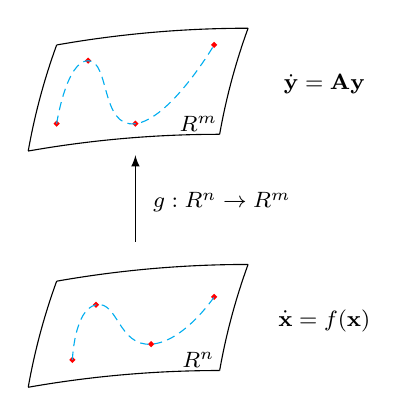
\begin{tikzpicture}
        
        \begin{scope}[shift={(0,0)}, scale=2]
            \draw[name path=path1] (0,0)  arc (100:90:7) coordinate(A);
            \draw[name path=path2] (0,0) arc (160:170:4) coordinate(B);
            \draw[name path=path3] (A) arc (160:170:4);
            \draw[name path=path4] (B) arc (100:90:7);

            \draw[red, thick, fill=red] (0,-0.5) coordinate(P1) circle (0.01);
            \draw[red, thick, fill=red] (0.2,-0.1) coordinate(P2) circle (0.01);
            \draw[red, thick, fill=red] (0.5,-0.5) coordinate(P3) circle (0.01);
            \draw[red, thick, fill=red] (1,0) coordinate(P4) circle (0.01);

            \draw[cyan, densely dashed] plot [smooth, tension=1] coordinates { (P1) (P2) (P3) (P4)};
            \node at (0.9,-0.5) {\footnotesize $\mathbb{R}^m$};
            \node at (1.7, -0.25) {\footnotesize $\dot{\mathbf{y}}=\mathbf{A}\mathbf{y}$};
        \end{scope}
        
        \draw[-latex] (1,-2.5) -- (1,-1.4);
        \node[anchor=west] at (1.1,-2) {\footnotesize $g:\mathbb{R}^n \to \mathbb{R}^m$};

        \begin{scope}[shift={(0,-3)}, scale=2]
            \draw[name path=path1] (0,0)  arc (100:90:7) coordinate(A);
            \draw[name path=path2] (0,0) arc (160:170:4) coordinate(B);
            \draw[name path=path3] (A) arc (160:170:4);
            \draw[name path=path4] (B) arc (100:90:7);
            % circle around the node
            \draw[red, thick, fill=red] (0.1,-0.5) coordinate(P1) circle (0.01);
            \draw[red, thick, fill=red] (0.25,-0.15) coordinate(P2) circle (0.01);
            \draw[red, thick, fill=red] (0.6,-0.4) coordinate(P3) circle (0.01);
            \draw[red, thick, fill=red] (1,-0.1) coordinate(P4) circle (0.01);

            \draw[cyan, densely dashed] plot [smooth, tension=1] coordinates { (P1) (P2) (P3) (P4)};
            \node at (0.9,-0.5) {\footnotesize $\mathbb{R}^n$};
            \node at (1.7, -0.25) {\footnotesize $\dot{\mathbf{x}}=f(\mathbf{x})$};
        \end{scope}
    \end{tikzpicture}
    \end{adjustbox}
    \caption{Some description}
    \label{fig:koopman}
  \end{figure}
\end{frame}

%---------------------------------------------------------

\begin{frame}\frametitle{TikZ Keviats}
  Well, tikz is AWESOME, however as you probably noticed by now, it can take a lot of time compiling the whole document if it contains multiple tikzpictures.
  
  If possible, generate the tikzpictures in a standalone file, i.e., generate .pdf files with the figures and only import those to the main file. Believe me, it will reduce by a lot the time you spend waiting for the compiled file.
\end{frame}

%---------------------------------------------------------
\section{Useful Features}
%---------------------------------------------------------

\begin{frame}\frametitle{Equations}
  Since this is latex, we can use equations.

  \vspace{0.2cm}

  % example
  \begin{equation}
    \dot{\mathbf{x}} = \mathbf{A}\mathbf{x} + \mathbf{B}\mathbf{u}
  \end{equation}

  \vspace{0.2cm}

  All equations are numbered by the order they appear in the presentation. But if you don't want a numbered equation, you can still do it

  \vspace{0.2cm}
  
  \begin{equation*}
    E = mc^2
  \end{equation*}
\end{frame}


%--------------------------------------------------------
 
\begin{frame}\frametitle{Blocks}

  \centering
  \begin{minipage}{0.7\linewidth}
    One useful and nice feature is the block environment (\textit{newtheorem}). It can be used to highlight important information. (see preamble.tex)
  
  

  \vspace{0.5cm}

  \begin{conferences}
    \begin{enumerate}
      \item American Control Conference, Toronto, July 2024 \\ Initial deadline: \textbf{September 22, 2023}
      \item European Control Conference, Stockholm, June 2024 \\ Initial deadline: \textbf{October 25, 2023}
    \end{enumerate}
  \end{conferences}

  \begin{theorem}[Theorem name]
    This is a theorem. % smily face
  \end{theorem}
  \begin{remark}
    This is a remark.
  \end{remark}

  \end{minipage}
\end{frame}

%--------------------------------------------------------

\begin{frame}[t]\frametitle{Include figures}
  \begin{minipage}[t]{0.48\textwidth}
    \begin{figure}[H]
    \includegraphics[width=0.85\linewidth]{example-image-a}
    \caption{Caption 1}
    \end{figure}

  \end{minipage}%
  \begin{minipage}{0.05\textwidth}
    \hfill
  \end{minipage}%
  \begin{minipage}[t]{0.48\textwidth}	  
    \begin{figure}
    \includegraphics[width=0.85\linewidth]{example-image-b}
    \caption{Caption 2}
    \end{figure}
  \end{minipage}
\end{frame}

%--------------------------------------------------------

\begin{frame}\frametitle{Insert videos}
    \begin{center}  
      % \movie from the multimedia package is incompatible with Tectonic (XeTeX).
      % We replace it with \href{run:...} which compiles correctly and is supported by pdfpc.
      \href{run:figures/apollo17.avi}{\includegraphics[width=0.5\textwidth, height=0.3\textwidth]{example-image-c}}
    \end{center}
    \vspace{0.5cm}
    Note that only some pdf viewer can render the video. For presentions I recommend using `\textit{pdfpc}', an open source presentation viewer that mimics the presentation layout from PowerPoint (some advantages include a timer, a way to see the next slide before it is presented and the use of a pointer or a pen)
\end{frame}


%--------------------------------------------------------

\begin{frame}\frametitle{Citations}
  Just as a normal .tex document we can use .bib files to cite references. 
  \vspace{0.5cm}
  \begin{itemize}
    \item Some random text\ldots~\cite{Smith1986}
    \item Another random text\ldots~\cite{
      Parrilo2003, Muldowney1990}
  \end{itemize}

  \vspace{0.5cm}
  The references are shown at the end of the presentation automatically. 
  
\end{frame}

%--------------------------------------------------------

\begin{frame}\frametitle{Bibliography}
  
  In the next slide, you have the default final slide. You can edit it as you see fit. 

  In the current state you just need to change the photo and a few information details.
\end{frame}


%--------------------------------------------------------
% Biography and last slide
%--------------------------------------------------------
%---------------------------------------------------------
% Biography slide (not used in this template)
% Instead just upload a pdf file with your biography from
% powerpoint or keynote with the name Profile.pdf
%---------------------------------------------------------

\begin{frame}[plain]

    \begin{tikzpicture}[overlay, remember picture]
      \clip (current page.north west) rectangle (current page.south east);
      \shade[%
        top color= renatoSblue!70!white,
        bottom color= renatoSblue,
        shading angle=-45,
        opacity=1
        ]
        (current page.north west) rectangle (current page.south east);
        
        \node[anchor=north west] at ([xshift=1cm, yshift=-1cm]current page.north west) {\pgfuseimage{unilogow}};
        \node[text=white, anchor=north west] at ([xshift=2.25cm, yshift=-1.75cm]current page.north west)
            {Institute of Flight Mechanics and Controls};
    

        \node[text=white, font=\Large\bfseries, anchor=north west] at ([xshift=1cm, yshift=-3cm]current page.north west) {Thank you!};


      % This is the node to change the picture, just change the file specified for the speaker image
        \node[circle, draw, opacity=1, color=white , minimum size=2.5cm, path picture={
        \node at (path picture bounding box.center){\pgfuseimage{speaker}};}] at ([xshift=2.3cm, yshift=-5cm]current page.north west) {};
              
      % This is the node to change the information 

      \node[text=white, anchor=north west, align=left] at ([xshift=4cm, yshift=-3.8cm]current page.north west){
        \insertbioINFO
      };
        
    \end{tikzpicture}
\end{frame}

% -------------------------------------------------------
% Bibliography
% Just remove the comment if you want to include a reference 
% slide
% -------------------------------------------------------

\begin{frame}[allowframebreaks]
    \frametitle{References}
    \bibliographystyle{unsrt}    % sorted (appears in order of citation)
    \bibliography{utils/references.bib}
\end{frame}

% -------------------------------------------------------
% Appendix
% -------------------------------------------------------

%%---------------------------------------------------------
% Appendix slides
% Not presented in the root.pdf file
%---------------------------------------------------------

\begin{frame}[plain]
    
    \begin{tikzpicture}[overlay, remember picture]
        \clip (current page.north west) rectangle (current page.south east);
      \shade[%
        top color= renatoSblue!70!white,
        bottom color= renatoSblue,
        shading angle=-45,
        opacity=1
        ]
        (current page.north west) rectangle (current page.south east);
      \end{tikzpicture}
    
    \begin{tikzpicture}    
        \node[text width=3.5cm, opacity=1] at (0,-1) {\textcolor{white}{\Huge{{\fontsize{50}{60}\selectfont Appendix}}}};
    \end{tikzpicture}
    
\end{frame}

\appendix

%---------------------------------------------------------
\section{Appendix}
%---------------------------------------------------------

%---------------------------------------------------------
\begin{frame}\frametitle{Appendix}


\end{frame}




\end{document}